\documentclass[12pt,]{article}
\usepackage{lmodern}
\usepackage{amssymb,amsmath}
\usepackage{ifxetex,ifluatex}
\usepackage{fixltx2e} % provides \textsubscript
\ifnum 0\ifxetex 1\fi\ifluatex 1\fi=0 % if pdftex
  \usepackage[T1]{fontenc}
  \usepackage[utf8]{inputenc}
\else % if luatex or xelatex
  \ifxetex
    \usepackage{mathspec}
  \else
    \usepackage{fontspec}
  \fi
  \defaultfontfeatures{Ligatures=TeX,Scale=MatchLowercase}
\fi
% use upquote if available, for straight quotes in verbatim environments
\IfFileExists{upquote.sty}{\usepackage{upquote}}{}
% use microtype if available
\IfFileExists{microtype.sty}{%
\usepackage{microtype}
\UseMicrotypeSet[protrusion]{basicmath} % disable protrusion for tt fonts
}{}
\usepackage[margin=1in]{geometry}
\usepackage{hyperref}
\PassOptionsToPackage{usenames,dvipsnames}{color} % color is loaded by hyperref
\hypersetup{unicode=true,
            pdftitle={The Thresholding Bandit Problem},
            pdfauthor={Tim Radtke},
            colorlinks=true,
            linkcolor=Maroon,
            citecolor=Blue,
            urlcolor=blue,
            breaklinks=true}
\urlstyle{same}  % don't use monospace font for urls
\usepackage{graphicx,grffile}
\makeatletter
\def\maxwidth{\ifdim\Gin@nat@width>\linewidth\linewidth\else\Gin@nat@width\fi}
\def\maxheight{\ifdim\Gin@nat@height>\textheight\textheight\else\Gin@nat@height\fi}
\makeatother
% Scale images if necessary, so that they will not overflow the page
% margins by default, and it is still possible to overwrite the defaults
% using explicit options in \includegraphics[width, height, ...]{}
\setkeys{Gin}{width=\maxwidth,height=\maxheight,keepaspectratio}
\IfFileExists{parskip.sty}{%
\usepackage{parskip}
}{% else
\setlength{\parindent}{0pt}
\setlength{\parskip}{6pt plus 2pt minus 1pt}
}
\setlength{\emergencystretch}{3em}  % prevent overfull lines
\providecommand{\tightlist}{%
  \setlength{\itemsep}{0pt}\setlength{\parskip}{0pt}}
\setcounter{secnumdepth}{5}
% Redefines (sub)paragraphs to behave more like sections
\ifx\paragraph\undefined\else
\let\oldparagraph\paragraph
\renewcommand{\paragraph}[1]{\oldparagraph{#1}\mbox{}}
\fi
\ifx\subparagraph\undefined\else
\let\oldsubparagraph\subparagraph
\renewcommand{\subparagraph}[1]{\oldsubparagraph{#1}\mbox{}}
\fi

%%% Use protect on footnotes to avoid problems with footnotes in titles
\let\rmarkdownfootnote\footnote%
\def\footnote{\protect\rmarkdownfootnote}

%%% Change title format to be more compact
\usepackage{titling}

% Create subtitle command for use in maketitle
\newcommand{\subtitle}[1]{
  \posttitle{
    \begin{center}\large#1\end{center}
    }
}

\setlength{\droptitle}{-2em}
  \title{The Thresholding Bandit Problem}
  \pretitle{\vspace{\droptitle}\centering\huge}
  \posttitle{\par}
  \author{Tim Radtke}
  \preauthor{\centering\large\emph}
  \postauthor{\par}
  \predate{\centering\large\emph}
  \postdate{\par}
  \date{4/23/2017}

\usepackage[retainorgcmds]{IEEEtrantools}
\usepackage{bm}
\usepackage{amsmath}
\usepackage{bbm}
\newtheorem{theorem}{Theorem}
\newcommand{\KL}{\,\text{KL}}
\newcommand{\der}{\,\text{d}}

\begin{document}
\maketitle

The \emph{Thresholding Bandit Problem} described in Locatelli et al.
(2016) can be considered a variant of a variant. It can be framed into
the wider literature of \emph{Pure Exploration} multi-armed bandit
problems. In particular, it shares characteristics with the
\emph{Top-\(m\)} problem. This problem is concerned with finding the
\(m\) best arms as described by the means of their corresponding
distributions. This in turn is similar to the \emph{combinatorial
bandit} problem, which also aims at finding the \(m\) best arms.
However, it is able to pull several arms at once: Think of an online
shop that shows five recommended products on a product detail page.
These five recommended products might each be represented by an arm, and
we look for the products with the largest mean conversion rate. The
thresholding bandit problem we discuss here, however, is concerned with
pulling a single arm at a time. And so a more appropriate situation is
that of a website presenting a banner. Again, think of an online shop
trying to promote a certain category. The content team came up with a
number of different designs for the banner, and it's not clear how many
click-throughs they will gather.

The idea now is that we would like to classify the banners into two
distinct groups: A group with a mean conversion rate \(\mu_i\) below
threshold \(\tau\), and a group with mean conversion rate \(\mu_i\)
above threshold \(\tau\). This might be the optimization problem when we
are concerned with not falling below a certain minimum level
click-through rate with the banners we're choosing.

If it turns out that in general we can find relatively quickly whether
arms are above or below a threshold, then this kind of test can be used
to safeguard against very bad versions in a test. Before we move to a
Top-\(m\) test, we might want to run a thresholding version and then
continue only with the arms classified into the group above the
threshold. This might be justified when adjusting parts of the checkout
process of an online shop, where the conversion rate or the average
order value should not drop below a threshold.

\subsection{Setup}\label{setup}

In any case, the problem boils down to the following. As standard in
multi-armed bandit problems, we have \(K\) arms
\(\mathcal{A} = \{1, \dots K\}\). We can pull arm \(k\) at time \(t\) to
collect feedback in form of the random variable \(X_{k,t}\) which is
distributed accoring to the arm's distribution \(\nu_k\). In general, we
are concerned with estimating for each arm \(i\) the mean \(\mu_i\) of
its distribution \(\nu_i\). In contrast to most bandit problems,
however, we do not directly compare arms with each other by comparing
their means. In the case of pure exploration bandits, it is for example
necessary to compare the arms because one aims to find the best one. In
the case of the thresholding bandit, however, we compare each arm's mean
\(\mu_i\) individually against the threshold \(\tau \in \mathbb{R}\)
which is known and fixed before the experiment. One might compare this
to a pure exploration bandit in which the mean of the best arm is known
upfront. We will see later that this fact leads to advantages in the
design of algorithms which are not as readily available in other bandit
settings.

In Locatelli (2016), the arms' distributions are assumed to follow a
\(R\)-sub-Gaussian distribution. Under this assumption, the authors are
able to proof a general lower bound as well as an algorithm with a
matching upper bound. Both hinge upon the \emph{complexity} of a given
problem. Since bandit problems can differ in the number of the arms
\(K\) and the means of each arm, some pose easier identification
problems than others. Indeed, in the thresholding problem, the
difficulty of the problem naturally depends on how close (the means of
the) distributions are to the fixed threshold. Intuitively, the closer a
mean \(\mu_i\) is to the threshold \(\tau\), the more difficult it will
be to distinguish the two successfully based on samples from the
distribution \(\nu_i\). For the case of the sub-Gaussian distributions,
a natural measure of this distance is given by simply
\(\Delta_i = |\tau - \mu_i| + \epsilon\), where \(\epsilon\) defines a
\(2\epsilon\) interval around the threshold \(\tau\) in which we allow
ourselves to make a mistake at no cost.

If we extend this idea to the set of arms \(i \in \{1,...,K\}\) of a
given bandit problem, a natural measure of the overall diffulty of the
problem, or the problem's complexity, might be given by
\(H = \sum_{i=1}^{K} \Delta_i^{-2}\). In particular, it shows that just
adding additional arms leads to an increase in complexity (since we need
to sample more of them), just as smaller \(\Delta_i\) will increase the
complexity as arms become harder to classify. (WHERE DOES THIS
COMPLEXITY ORIGINALLY COME FROM? WHAT IS ITs MOTIVATION? ITS NOT THAAAT
NATURAL)

We also see that this definition may lose relevancy as we move away from
\(R\)-sub-Gaussian distributions. (ADD QUICK EXAMPLE OF WHAT CHANGES;
REFER TO LATER PART AND DESCRIBE THIS AS THE MOTIVATION OF THE PAPER)

Another characteristic uniquely identifying bandit problems is the
regret measure that we aim to optimize. As explained during the
introduction, multi-armed bandits traditionally optimize cumulative
regret. The notion of regret considered in the thresholding bandit,
however, is more akin to the regret in pure exploration bandits or the
error probability in sequential hypothesis testing. Indeed, one can most
easily describe the regret in the thresholding case as the probability
of making a misclassification of any arm. Or, more rigorously, let us
define the set of all arms with mean larger than the threshold,
\(\mathcal{S}_\tau = \{i \in \mathcal{A}: \mu_i \geq \tau\}\).
Consequently,
\(\mathcal{S}_\tau^C = \{i \in \mathcal{A}: \mu_i < \tau\}\). At the end
of the sampling rule/procedure (!!we have not mentioned yet the fact
that we're in the fixed budget case!!), we demand that any algorithm
returns the two corresponding \emph{estimated} sets:
\(\hat{\mathcal{S}}_{\tau} = \{i \in \mathcal{A}: \hat{\mu}_i \geq \tau\}\),
as well as
\(\hat{\mathcal{S}}_{\tau}^C = \{i \in \mathcal{A}: \hat{\mu}_i < \tau\}\).
We simply demand an answer to the question which arms have means above
the threshold \(/tau\), and which arms lie below \(\tau\). Let \(T\) be
the overall number of samples the algorithm is allowed to pull. We
define the loss as
\(\mathcal{L}(T) = \mathbbm{1}_{\{\hat{\mathcal{S}}_{\tau} \cap \mathcal{S}_{\tau-\epsilon}^C \neq \emptyset\}} \cdot \mathbbm{1}_{\{\hat{\mathcal{S}}_{\tau}^C \cap \mathcal{S}_{\tau+\epsilon} \neq \emptyset\}}\).
That is, we compare the return set with the true set and collect a loss
of 1 if any arm with a true mean outside the \(2\epsilon\) interval
around \(\tau\) was misclassified. It is important to realize that arms
with means inside the \(2 \epsilon\) interval may be misclassified
without it affecting the loss. These arms are considered close enough to
the threshold that we do not care whether they lie above or below.

ADD A GRAPHIC THAT VISUALIZES THE ESTIMATED AND THE REQUIRED RETURN SETS

From there, it is natural to define the expected regret/loss as
\(\mathbb{E}[\mathcal{L}(T)] = \mathbb{P}((\hat{\mathcal{S}}_{\tau} \cap \mathcal{S}_{\tau-\epsilon}^C \neq \emptyset) \land (\hat{\mathcal{S}}_{\tau}^C \cap \mathcal{S}_{\tau+\epsilon} \neq \emptyset))\).
This, of course, is the mentioned probability of making a mistake.

ADD REMARK ON WHAT THIS IMPLIES WITH REGARD TO THE MEANS

Lastly, it is to mention that we are considering the fixed-budget
version of the thresholding bandit problem. We thus fix the number of
samples that the algorithm will pull upfront at \(T\). The task of the
algorithm is then to find a sampling rule or strategy which distributes
the budget \(T\) among the \(K\) arms in such a way that the expected
regret, or the error probability, is minimized. In other terms, the
algorithm aims to use the \(T\) samples in a way that lets him return
the two sets \(\hat{\mathcal{S}}_{\tau}\) and
\(\hat{\mathcal{S}}_{\tau}^C\) with as much confidence as possible. This
again shows the contrast to the fixed confidence setting in which one
fixes the confidence level upfront and lets the algorithm draw as many
samples as necessary to reach the required confidence.

At this point, we have defined the fixed budget thresholding bandit
setup for any algorithm in the case of sub-Gaussian distributions. We
thus proceed to describe the algorithm proposed in Locatelli et al.
(2016).

\subsection{The APT Algorithm}\label{the-apt-algorithm}

In the following we describe the \emph{Anytime Parameter-free
Thresholding} (APT) algorithm proposed in Locatelli et al. (2016), which
is a simple yet effective algorithm and displays some very favorable
characteristics when compared with alternative algorithms.

From the general setup, we already know how the algorithm will end.
After it has drawn \(T\) samples, the algorithm makes its decision of
which arms to include in the return sets solely on basis of the
empirical means \(\hat{\mu}_i(T)\) estimated until time \(T\).
Furthermore, the threshold and interval around the threshold were fixed
upfront and serve as argument to the algorithm: \((\tau, \epsilon)\).
For a given arm \(i\) and a given time \(t\), we let \(T_i(t)\)
represent the number of samples drawn from arm \(i\) until time \(t\)
(including). Consequently, the empirical mean of arm \(i\) at time \(t\)
is given by \(\mu_i = \frac{1}{T_i(t)} \sum_{s=1}^{T_i(t)} X_{i,s}\)
where \(X_{i,s}\) is the feedback sampled from distribution \(\nu_i\)
when the arm is pulled for the \(s\)-th time.

To be specific, the APT algorithm initiates by pulling each arm once.
Then, for each \(t > K\), it calculates for every arm the values
\(T_i(t)\) and \(\mu_i(t)\). Based on the empirical mean, the algorithm
computes the estimated gap between the mean and the threshold as
\(\hat{\Delta}_i(t) = \hat{\Delta}_i^{\tau, \epsilon}(t) = |\mu_i(t) - \tau| + \epsilon\).
The decision of which arm is sampled next is then based on the value
\(B_i(t+1) = \sqrt{T_i(t)} \hat{\Delta}_i(t)\): the algorithm pulls arm
\(I_{t+1} = \arg \min_{i\leq K} B_i(t+1)\) minimizing this decision
quantity. After \(T\) pulls overall, the arm returns the sets described
in the general setup, \(\hat{\mathcal{S}}_{\tau}\) and
\(\hat{\mathcal{S}}^C_{\tau}\).

\textbf{Remark}: Obviously, the APT algorithm tends to pull arms more
often with corresponding mean close to the threshold and interval (small
\(\hat{\Delta}_i(t))\). This makes sure that more evidence is gathered
on arms which appear to be inherently difficult to classify based on the
samples collected until time \(T_i(t)\), as these arms stifle the
confidence the most. That is, until we have collected enough evidence to
make a confident classification even if the mean is truly close to the
threshold. In that case, \(\sqrt{T_i(t)}\) will raise \(B_i(t+1)\).
Consequently, other arms farther away from the threshold will be sampled
again. In this way, the algorithm tries to distribute the budget \(T\)
over all arms so as to define a sampling rule optimizing the confidence
of the final decision. Of course, that's just Glivenko-Cantelli and the
CLT making sure \(B_i(t+1)\) is not degenerate.

\subsection{Discussion}\label{discussion}

One of the APT algorithm's main features is its simplicity. The sampling
rule is very straightforward, and, as highlighted in Locatelli et al.
(2016), it does not require any knowledge about the type of
sub-Gaussianity \(R\), or the complexity \(H\) upfront. This makes the
algorithm immediately applicable in practice while it still enjoys its
upper bound on the expected regret. This is in particular worth
highlighting when comparing APT to algorithms used in the pure
exploration bandit setting. There, many algorithms require knowledge
about the corresponding complexity upfront. The problem however being,
that to know the complexity, the experimenter has to know all means up
to a permutation of the arms (for example, see Audibert et al., 2010).
This, of course, is not given in practice and thus alternative
algorithms try to estimate the complexity online which is not a
desirable solution either as especially in the beginning plug-in
estimates based on the estimated means may lead to wrong estimates of
the complexity and consequently budget allocation based on mistaken
beliefs (compare Garivier and Kaufmann, 2016).

Furthermore, Locatelli et al. (2016) were able to present an upper bound
for the APT algorithm matching the lower bound in their Theorem 1.
Proofs of both bounds are given below.

Where the APT algorithm shows room for improvement is when it comes to
settings with distributions that are not sub-Gaussian. This is mentioned
in Locatelli et al. (2016). In general, the problem becomes that the
assumptions for the bounds no longer hold; furthermore, the statistic
\(B_i(t+1)\), and the term \(\hat{\Delta_i}(t)\) are motivated by
(sub-)Gaussian distributions. The more one moves away from Gaussian-like
distributions, the less appropriate this term becomes, however. In
particular, the empirical mean will be less concentrated around the true
mean and more impacted by outliers which are more likely under non
sub-Gaussian distributions. Locatelli et al. (2016) thus refers to
Bubeck et al. (2013) which considers solutions for multi-armed bandits
that are based on heavy-tail distributions. By using more robust
estimators of the mean, one could equip the APT algorithm to deal with
such distributions.

Another step towards dealing with non sub-Gaussianity is made by
Mukherjee et al. (2017) who use an estimate of the variance additionally
to the empirical mean in their Augmented UCB solution. Utilizing this
additional information, the algorithm seems to perform better than for
example APT, going from simulation results displayed in the paper. We
will continue to discuss the Augmented UCB solution further in chapter
3.

Yet another idea, again mentioned in Locatelli et al. (2016) is to show
bounds based on the Kullback-Leibler divergence of the specific
distribution directly. While the approximation through the Gaussian
Kullback-Leibler divergence in the lower bound proof is convenient and
leads to the simple APT algorithm, it might not stay appropriate for
distributions whose Kullback-Leibler divergence tends to differ from the
Gaussian. This, for example, is the case for Bernoulli distributions at
very small parameters \(\mu\). It's quite obvious simply by looking at
examples that the Kullback-Leibler divergence of Bernoullis starts to
lose any similarity to the plain quadratic approximation. The second
graph then shows, that the actual Kullback-Leibler divergence of
Bernoullis also has lost any symmetry over this range of parameter
values. Given that Bernoulli distributions with very small parameter
values arise naturally in many applications in website optimization and
advertising click-through modeling, there is a need to tackle this
problem.

Refer also to page 6 in Kaufmann et al. (2016): ``This
information-theoretic lower bound permits to interpret the quantity
\(H(\nu)\) defined in (2) as a subgaussian approximation''.

And so a potential approach can be to use the Kullback-Leibler
divergence as measure similar to the methods proposed in Kaufmann et al.
(2015). They proposed Kullback-Leibler based approaches for the pure
exploration bandit setting, which we will describe in chapter 2. Then,
in chapter 3, we will come back to the problem of using the
Kullback-Leibler divergence in the thresholding bandit setting.

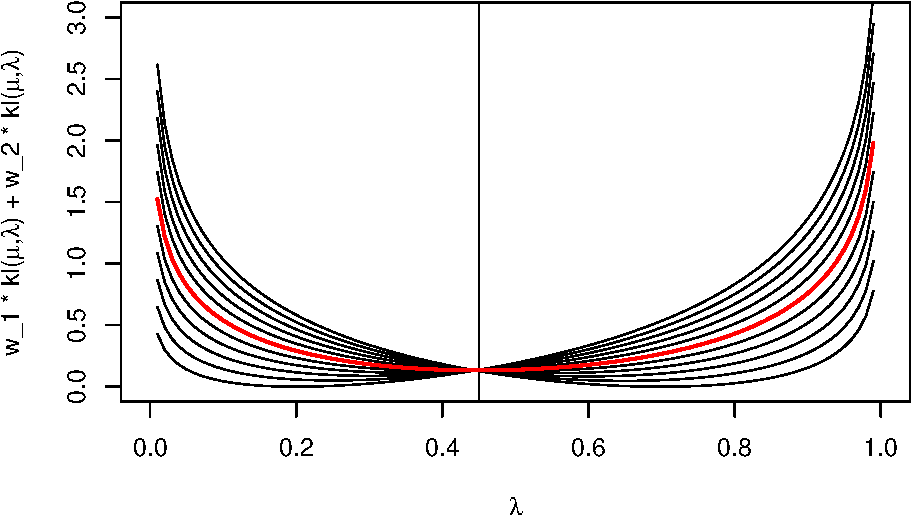
\includegraphics{ThresholdingBandit_files/figure-latex/unnamed-chunk-1-1.pdf}

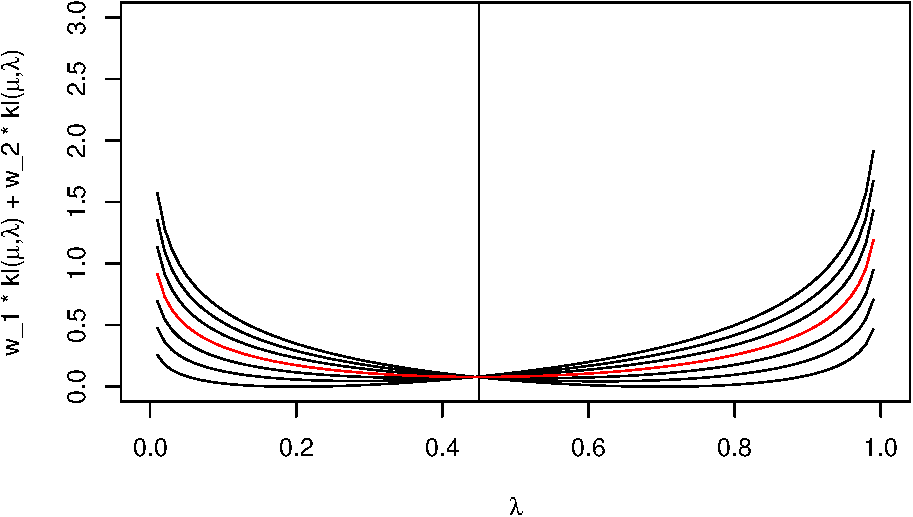
\includegraphics{ThresholdingBandit_files/figure-latex/unnamed-chunk-2-1.pdf}


\end{document}
